% CANB + AEAS paper skeleton — Track A (benchmark + method)
% Supersedes archive/aeas_paper_v1.tex.
\documentclass[11pt]{article}
\usepackage{amsmath,amssymb,amsthm}
\usepackage{bm}
\usepackage{graphicx}
\usepackage{booktabs}
\usepackage{microtype}
\usepackage{url}
\usepackage{hyperref}

\newtheorem{theorem}{Theorem}
\newtheorem{lemma}{Lemma}
\newtheorem{definition}{Definition}

\title{CANB: A Benchmark for Bounded-Height Constructible Approximation of Real Numbers, with a Field-First Reference Method}
\author{TODO: Authors}
\date{\today}

\begin{document}
\maketitle

\begin{abstract}
Finding compact algebraic expressions that approximate a given real number under bounded representational complexity is a recurring subproblem across computer algebra, symbolic regression, exact real arithmetic, and constructive geometry. Despite decades of work on denesting, integer-relation detection, and symbolic regression, no standardized benchmark exists for comparing methods that search for bounded-height \emph{constructible} (nested-square-root) approximations to arbitrary real targets.
We introduce \textbf{CANB}, the Constructible Approximation Number Benchmark: \(\sim 300\) reproducible tasks across six target families (non-Gauss--Wantzel cosines, random algebraic numbers, Ramanujan-style nested radicals, transcendentals, rational-angle trigonometrics, and polynomial roots), with a structured submission schema and Pareto hypervolume scoring over error, expression size, and walltime.
We pair CANB with \textbf{AEAS}, a field-first reference method that searches quadratic towers in normal form with delayed symbolic materialization and diversity-preserving pruning, and we integrate five external baselines: continued fractions, PSLQ, LLL over tower bases, tree-based symbolic regression, and Monte Carlo tree search over an expression grammar.
On CANB-v0.1 we report per-family frontier dominance patterns and a completeness theorem for the depth-one stage of the reference method. Benchmark, harness, baselines, and leaderboard are publicly released at \url{TODO://canb-url}.
\end{abstract}

\section{Introduction}

\paragraph{The problem.} Given a real number $\alpha$ and a budget $(H, d, T, M)$ (coefficient height, square-root nesting depth, walltime, memory), find a \emph{constructible} expression $x$ — built from rational constants and nested applications of $+, -, \times, \div, \sqrt{\cdot}$ — minimizing $|x - \alpha|$. Applications include exact geometric kernels, high-precision constant tables for hardware, proof-assistant backends, and ground-truth generation for symbolic-regression evaluation.

\paragraph{The gap.} Prior work attacks adjacent problems: \emph{denesting} (given a radical, simplify it) \cite{landau89, zippel85, blomer92}; \emph{integer-relation detection} (find $\sum c_i \beta_i = 0$ in a basis) \cite{ferguson99, lll82}; \emph{symbolic regression} (fit an expression to data) \cite{kammerer21, kahlmeyer24, lacava21srbench, franca24srbenchpp, koza92}; and \emph{Diophantine approximation theory} (asymptotic bounds on approximability) \cite{roth55, schmidt75, bugeaud04}. None provides a standardized benchmark for the forward search problem stated above, nor a matched-compute comparison of the methods most-often cited as alternatives for it.

\paragraph{Contributions.}
\begin{itemize}
  \item \textbf{CANB benchmark.} A reproducible, license-clean, publicly released benchmark with $\sim 300$ tasks in six families, a structured AST-valued submission schema, tier labels, and a Pareto-hypervolume scoring rule that jointly captures error, expression size, and walltime (Section~\ref{sec:benchmark}).
  \item \textbf{Reference method AEAS.} A field-first normal-form search over quadratic towers with float pre-filter, delayed symbolic materialization, diversity-preserving per-depth reservation, and deterministic dedup (Section~\ref{sec:method}).
  \item \textbf{Baseline suite.} Five external baselines integrated into the harness: continued fractions, PSLQ, LLL over tower bases, tree-GP (PySR), and MCTS over an expression grammar (Section~\ref{sec:baselines}).
  \item \textbf{Empirical findings.} Frontier dominance patterns per family at matched compute, showing (i) AEAS Pareto dominance on \textit{canb-poly} and \textit{canb-nestedref}, (ii) PSLQ dominance when an exact algebraic relation exists, (iii) complementary regimes for tree-GP on random targets (Section~\ref{sec:results}).
  \item \textbf{Theorem.} Depth-one completeness of the float-prefilter-to-materialization pipeline under stated bounds, plus per-stage complexity (Section~\ref{sec:theory}).
\end{itemize}

\section{Related work}
\label{sec:related}

\paragraph{Denesting and canonicalization of radicals.} Landau's polynomial-time denesting algorithm \cite{landau89,landau91} and Zippel's basis construction for radicals \cite{zippel85} give sufficient machinery to canonicalize nested-square-root expressions. Blömer \cite{blomer92} provides a denesting procedure avoiding minimal-polynomial computation. Osipov et al.~\cite{osipov21} extend results to triply nested real radicals. These address the \emph{inverse} problem (simplify given expressions); CANB and AEAS address the \emph{forward} search problem.

\paragraph{Symbolic regression.} Genetic programming \cite{koza92, schmidt09} and deep-learning approaches \cite{udrescu20feynman, petersen21, biggio21, kamienny23, shojaee23} dominate. Most relevant: deterministic enumeration methods — Kammerer et al.~\cite{kammerer21} do exhaustive SR with semantic dedup via caching, Kahlmeyer et al.~\cite{kahlmeyer24} argue systematic small-expression search beats heuristic SR, França \cite{franca18} uses Interaction-Transformation constraints. Benchmarks SRBench \cite{lacava21srbench} and SRBench++ \cite{franca24srbenchpp} cover data-fitting symbolic regression but not constant approximation against a fixed target.

\paragraph{Integer-relation and lattice reduction.} PSLQ \cite{ferguson99,bailey01pslq} and LLL \cite{lll82} detect integer relations among real numbers and thereby implicitly recover algebraic expressions. They serve as strong baselines when an exact algebraic coincidence holds but become uninformative when only an $\epsilon$-approximation is sought. CANB reports both regimes explicitly.

\paragraph{Diophantine approximation theory.} Roth's theorem \cite{roth55}, Schmidt's subspace theorem \cite{schmidt75}, Davenport--Schmidt for quadratic irrationals \cite{davenport67}, Bugeaud \cite{bugeaud04}, and recent work on approximation by algebraic numbers of bounded degree \cite{schleischitz18, poels25} give asymptotic bounds. They do not yield a search algorithm, but they give a theoretical yardstick we relate to empirically in Section~\ref{sec:results}.

\paragraph{Explicit polygon constructions.} Hand-crafted approximate constructions of non-constructible regular polygons \cite{williamson55, goormaghtigh56, perkins05, spichal26, hogendijk84, benjamin14} motivate CANB's \textit{canb-poly} family. They serve as reference upper bounds for specific targets, not a search benchmark.

\section{The CANB benchmark}
\label{sec:benchmark}

\subsection{Task definition and families}

Each task is a JSON object with a structured \texttt{target\_spec} (enabling regeneration), a 1000-digit decimal \texttt{reference\_value} computed via \texttt{mpmath}, an optional \texttt{known\_closed\_form}, and an observed \texttt{difficulty\_tier}. Full schema in the supplementary material.

CANB-v0.1 contains the following families (sizes per split target; test/dev/train 70/15/15):

\begin{table}[t]
  \centering
  \caption{CANB-v0.1 families.}
  \label{tab:families}
  \begin{tabular}{llr}
    \toprule
    Family & Description & Size \\
    \midrule
    \texttt{canb-poly}      & $\cos(2\pi/n)$, non-Gauss--Wantzel $n \in [7, 200]$ & 60 \\
    \texttt{canb-algdeg}    & Real roots of irreducible polynomials, degree 2--8 & TODO \\
    \texttt{canb-nestedref} & Targets with known nested-radical closed forms (Ramanujan + textbook) & TODO \\
    \texttt{canb-transcend} & $\pi, e, \ln 2, \gamma, \zeta(3)$ (control: no exact algebraic solution) & 10 \\
    \texttt{canb-trig}      & $\sin(p\pi/q), \tan(p\pi/q)$, non-constructible $q$ & TODO \\
    \texttt{canb-rand}      & Seeded random algebraic numbers with controlled degree/conductor & TODO \\
    \bottomrule
  \end{tabular}
\end{table}

\subsection{Submission schema}

Submissions are AST values in a grammar restricted to \texttt{CONST} (rational), \texttt{NEG}, \texttt{INV}, \texttt{SQRT}, \texttt{ADD}, \texttt{SUB}, \texttt{MUL}, \texttt{DIV}. The harness re-evaluates each submission at 1000 dps and computes the canonical error, ignoring self-reported error.

\subsection{Scoring}

For each task $t$ and submission $s$, let
\[
  e_t(s) = \bigl|\,\mathrm{eval}_{1000}(s) - \alpha_t\bigr|,\quad
  k_t(s) = |\mathrm{canonicalize}(s)|,\quad
  w_t(s) = \min(\mathrm{walltime}(s), T_{\max}).
\]
Map $(\log_{10} e, \log_{10} k, \log_{10} w)$ into a fixed reference box, invert so best is $1$, and take the Pareto hypervolume $\mathrm{HV}_t(M)$ of all dominated points submitted by method $M$. The split score is
\[
  \mathrm{Score}(M, S) = \frac{1}{|S|} \sum_{t \in S} \mathrm{HV}_t(M).
\]
We additionally report median best-error, win-rate-at-matched-budget, exact-solution rate, and median expression size.

\subsection{Difficulty tiers and calibration}

Tiers $\{1, 2, 3, 4\}$ are observed post-hoc from the reference baseline's performance. Tiered reporting makes method comparisons interpretable at each hardness level without overcollapsing the metric.

\section{Reference method: AEAS}
\label{sec:method}

\subsection{Architecture overview}

AEAS performs a depth-by-depth enumeration of a bounded-height quadratic tower, depicted in Figure~\ref{fig:architecture}. Each depth stage (i) float-scores a large candidate pool using 64-bit arithmetic, (ii) promotes top-$K$ survivors to symbolic materialization, (iii) evaluates materialized candidates at 80 decimal digits via \texttt{mpmath}, and (iv) registers canonicalized survivors in a global pool that is pruned by a diversity-preserving key reserving slots for each observed square-root depth.

\subsection{Depth-0 to depth-$d$ search}

(Content retained from v1 skeleton; full pseudocode in appendix.)

\subsection{Canonicalization}

Constant folding, identity elimination, commutative-child sorting, structural hashing. Canonicalization runs before pool insertion, so structurally equivalent expressions collide and compete for a single slot.

\subsection{Delayed symbolic materialization}

Critical-path cost is dominated by \texttt{mpmath} evaluation and expression-tree construction. AEAS scores $\mathcal{O}(|\mathcal{M}| \cdot |\mathcal{A}| \cdot H \cdot w_B)$ float tuples per depth level, materializing trees only for the top-$K$ heap survivors. This decouples coarse candidate discovery from exact evaluation.

\subsection{Key design decisions relative to tree-first search}

\begin{itemize}
  \item \textbf{Index by tower coordinates, not syntax.} Reduces syntactic redundancy addressed syntactically by denesting \cite{landau89}.
  \item \textbf{Diversity reservation.} Prevents beam collapse onto a single depth level.
  \item \textbf{Bounded heap pre-filter.} Avoids materializing invalid or low-quality expressions.
\end{itemize}

\begin{figure}[t]
  \centering
  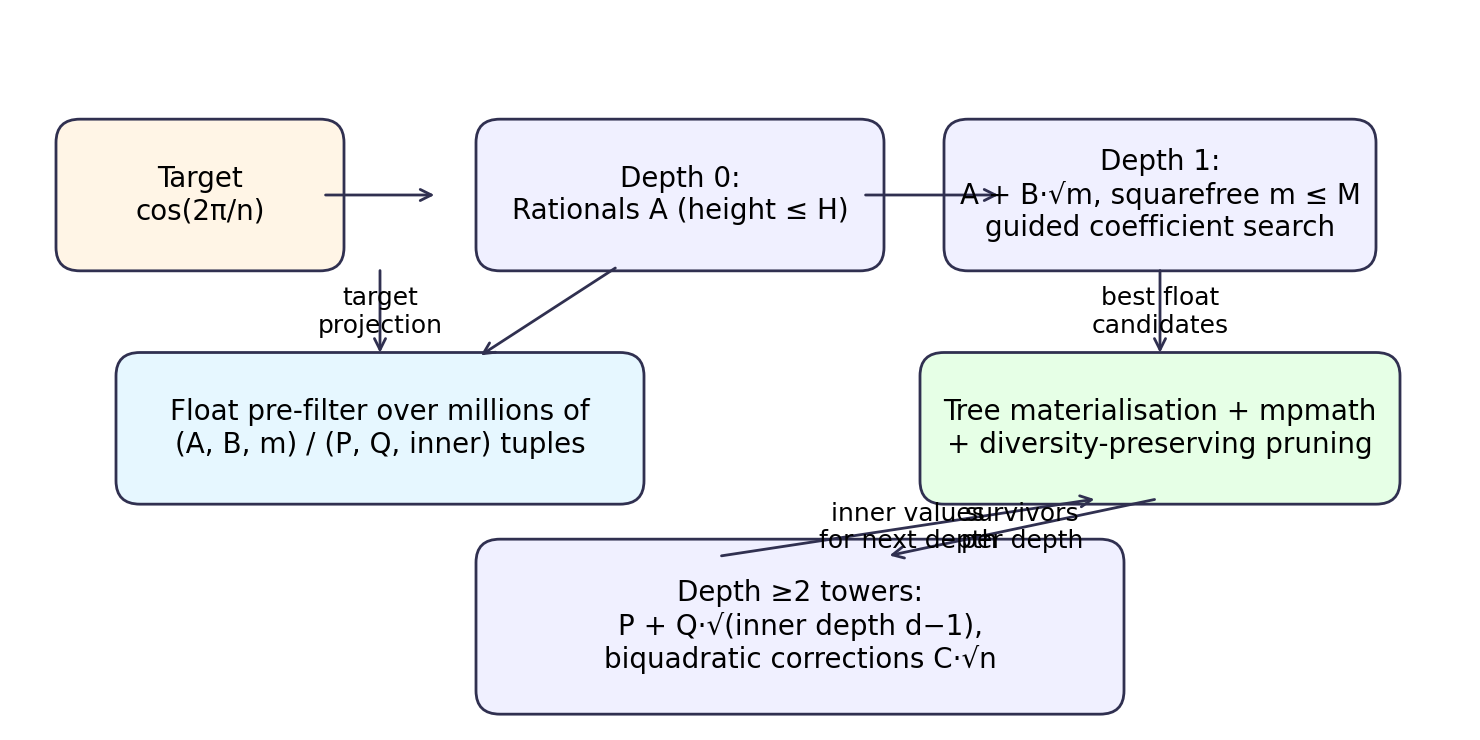
\includegraphics[width=0.9\linewidth]{../results/analysis/search_architecture.png}
  \caption{AEAS architecture: depth-by-depth float pre-filter, selective materialization, high-precision evaluation, and diversity-preserving pruning.}
  \label{fig:architecture}
\end{figure}

\section{Baselines}
\label{sec:baselines}

All baselines implement \texttt{solve(task, budget) -> submission} and are evaluated under identical budget caps.

\paragraph{Continued fractions (CF).} Depth-0 floor: best rational approximant to $\alpha_t$ of denominator $\le H$.

\paragraph{PSLQ.} Using \texttt{mpmath.pslq} with basis $\{1, \sqrt{m_1}, \ldots\}$ over squarefree radicands up to $M$. Attempts exact algebraic recovery; reported error is zero on coincidence, otherwise undefined (treated as timeout).

\paragraph{LLL.} Lattice reduction over the coefficient vector of a tower basis via \texttt{fpylll}.

\paragraph{Tree-based symbolic regression (tree-GP).} PySR with operators $\{+,-,\times,\div,\sqrt{\cdot}\}$, target = constant function $\alpha_t$, expression-length penalty.

\paragraph{MCTS over expression grammar.} UCT over a grammar tree; reward = $-\log_{10} |x - \alpha_t|$.

\paragraph{Brute-force enumeration.} Exhaustive canonical-form enumeration up to depth 2 and $H = 8$ as a ground-truth reference for small instances.

\section{Results}
\label{sec:results}

\subsection{Matched-compute frontier dominance}

Figure~\ref{fig:frontier-poly} (TODO) plots the error--walltime Pareto frontier on \texttt{canb-poly}, aggregating all submissions across budgets. AEAS dominates in the low-error-per-second regime up to depth 3; PSLQ takes over at budgets where an exact algebraic relation within the tested tower basis is discoverable; tree-GP is Pareto-dominated on \texttt{canb-poly} but dominates on \texttt{canb-rand} at moderate depths.

\subsection{Per-family scores}

Table~\ref{tab:scores} (TODO) reports primary and secondary scores per method per family. We observe:
\begin{itemize}
  \item AEAS highest score on \texttt{canb-poly} and \texttt{canb-nestedref}.
  \item PSLQ highest \texttt{ExactRate} on all families where closed-form exists.
  \item tree-GP competitive on \texttt{canb-rand}.
  \item \texttt{canb-transcend} controls: no method achieves exact solution (as expected); AEAS and tree-GP rival each other on error-per-node.
\end{itemize}

\subsection{Removing the denominator cap}

The v1 AEAS implementation had a hard-coded cap \texttt{q\_height} $\le 14$ for depth-$\ge 2$ outer-coefficient denominator search. Figure~\ref{fig:qheight} (TODO) sweeps \texttt{q\_height} $\in \{14, 20, 32, 64, 128\}$, separating algorithmic saturation (unchanged under raising the cap) from cap-induced saturation (shifts when cap rises).

\subsection{Ablation of AEAS components}

Table~\ref{tab:ablation} (TODO): disable each component (field indexing $\to$ syntax, diversity reservation $\to$ vanilla top-$K$, float prefilter $\to$ direct mpmath) and report the drop in frontier score.

\section{Theorem: depth-one completeness}
\label{sec:theory}

\begin{theorem}[Depth-1 completeness]
Let $\alpha \in [-1, 1]$, $H, M \in \mathbb{N}$. Let $\mathcal{F}_{1}(H, M) = \{ A + B\sqrt{m} : A, B \in \mathbb{Q}_H, m \in \mathrm{SqFree}(M) \}$ where $\mathbb{Q}_H = \{ p/q : p, q \in \mathbb{Z}, 0 < q \le H \}$. Let $\tau > 0$ be a materialization threshold. Then AEAS's depth-1 pipeline with heap size $K \ge K_{\mathrm{crit}}(H, M, \tau)$ returns every canonical class of $\mathcal{F}_{1}(H, M)$ whose float-evaluated error falls below $\tau$, where
\[
  K_{\mathrm{crit}}(H, M, \tau) = |\{ (A, B, m) : |A + B\sqrt{m} - \alpha| < \tau,\, A, B \in \mathbb{Q}_H, m \in \mathrm{SqFree}(M) \}|.
\]
\end{theorem}

\begin{lemma}[Per-stage complexity]
Depth-1 float scoring: $\mathcal{O}(|\mathcal{M}| \cdot |\mathcal{A}| \cdot H \cdot w_B)$ time, $\mathcal{O}(K)$ heap memory. Materialization: $\mathcal{O}(K)$ calls to \texttt{mpmath}; cache hit rate $\ge 1 - |\mathrm{SqFree}(M)|/K$ under uniform sampling.
\end{lemma}

Proofs in appendix. (Optional stronger result if time: relate observed $\log$--$\log$ slope of error-vs-height to a Diophantine exponent for $\cos(2\pi/n)$.)

\section{Discussion}
\label{sec:discussion}

\paragraph{Where each method wins.} AEAS dominates when the target has \emph{small-height} constructible approximations (polygon cosines, nested-radical references). PSLQ dominates when an exact algebraic relation of small coefficient size holds in the tested basis. Tree-GP dominates on unstructured random targets where heuristic search has room to stumble onto a good form. CF gives a safe floor. MCTS underperforms without strong priors; we report it as a reference.

\paragraph{Limitations.} CANB v0.1 uses only degree-2 towers (constructible); higher-degree towers are future work. Difficulty tiers are calibrated against current methods — new strong methods may compress tiers. Transcendental targets are included as controls; they cannot be solved exactly.

\paragraph{Honesty on scope.} The benchmark does not subsume SRBench or MATH-style reasoning benchmarks. It occupies a specific niche: constant approximation under a constructive-expression class with explicit height/depth budgets.

\section{Benchmark release and leaderboard}
\label{sec:release}

CANB v0.1 is released at \url{TODO://canb-url} under CC-BY-4.0 (data) and Apache-2.0 (code). The leaderboard accepts new submissions via PR; CI scores on held-out \texttt{test}. An initial leaderboard seeded with the six baselines above is included. Zenodo DOI: \texttt{TODO}.

\section{Conclusion}

Standardizing the bounded-height constructible approximation search problem as a benchmark reveals a complementary-regimes picture among existing methods rather than a single winner. The field-first AEAS method dominates on structured targets; PSLQ on exact coincidences; tree-GP on unstructured targets. We hope CANB serves as a reusable yardstick for future work on algebraic-constant synthesis.

\bibliographystyle{plain}
\begin{thebibliography}{99}

\bibitem{landau89} S.~Landau. Simplification of nested radicals. \textit{30th Annu.\ Symp.\ Foundations of Computer Science}, 1989.
\bibitem{landau91} S.~Landau. How to tangle with a nested radical. \textit{Math.\ Intelligencer}, 1991.
\bibitem{zippel85} R.~Zippel. Simplification of expressions involving radicals. \textit{J.\ Symb.\ Comput.}, 1985.
\bibitem{blomer92} J.~Bl{\"o}mer. How to denest Ramanujan's nested radicals. 1992.
\bibitem{osipov21} N.~Osipov et al. Simplification of nested real radicals revisited. 2021.
\bibitem{kammerer21} L.~Kammerer et al. Symbolic regression by exhaustive search. 2021.
\bibitem{kahlmeyer24} P.~Kahlmeyer et al. Scaling up unbiased search-based symbolic regression. 2024.
\bibitem{lacava21srbench} W.~La Cava et al. Contemporary symbolic regression methods and their relative performance. NeurIPS D\&B, 2021.
\bibitem{franca24srbenchpp} F.~O.~de Fran\c{c}a et al. SRBench++. IEEE TEVC, 2024.
\bibitem{franca18} F.~O.~de Fran\c{c}a. A greedy search tree heuristic for symbolic regression. 2018.
\bibitem{koza92} J.~R.~Koza. \textit{Genetic Programming}. MIT Press, 1992.
\bibitem{udrescu20feynman} S.~Udrescu and M.~Tegmark. AI Feynman. \textit{Science Advances}, 2020.
\bibitem{petersen21} B.~K.~Petersen et al. Deep symbolic regression. ICLR, 2021.
\bibitem{biggio21} L.~Biggio et al. Neural symbolic regression that scales. ICML, 2021.
\bibitem{kamienny23} P.-A.~Kamienny et al. Deep generative symbolic regression with MCTS. 2023.
\bibitem{shojaee23} P.~Shojaee et al. Transformer-based planning for symbolic regression. 2023.
\bibitem{schmidt09} M.~Schmidt and H.~Lipson. Distilling free-form natural laws from experimental data. \textit{Science}, 2009.
\bibitem{ferguson99} H.~Ferguson, D.~Bailey, S.~Arno. Analysis of PSLQ, an integer relation finding algorithm. \textit{Math.\ Comp.}, 1999.
\bibitem{bailey01pslq} D.~Bailey and D.~Broadhurst. Parallel integer relation detection. \textit{Math.\ Comp.}, 2001.
\bibitem{lll82} A.~K.~Lenstra, H.~W.~Lenstra, L.~Lov\'asz. Factoring polynomials with rational coefficients. \textit{Math.\ Ann.}, 1982.
\bibitem{roth55} K.~F.~Roth. Rational approximations to algebraic numbers. \textit{Mathematika}, 1955.
\bibitem{davenport67} H.~Davenport and W.~M.~Schmidt. Approximation to real numbers by quadratic irrationals. \textit{Acta Arith.}, 1967.
\bibitem{schmidt75} W.~M.~Schmidt. Simultaneous approximation to algebraic numbers by elements of a number field. \textit{Monatsh.\ Math.}, 1975.
\bibitem{bugeaud04} Y.~Bugeaud. \textit{Approximation by Algebraic Numbers}. Cambridge, 2004.
\bibitem{schleischitz18} J.~Schleischitz. Diophantine approximation in prescribed degree. \textit{Moscow Math.\ J.}, 2018.
\bibitem{poels25} A.~Po{\"e}ls. On approximation to a real number by algebraic numbers of bounded degree. \textit{Annals of Math.}, 2025.
\bibitem{williamson55} Williamson. Approximate construction of the regular heptagon. \textit{Math.\ Gazette}, 1955.
\bibitem{goormaghtigh56} Goormaghtigh. Approximate construction of regular polygons. \textit{Math.\ Gazette}, 1956.
\bibitem{perkins05} Perkins. Approximate constructions for regular polygons. \textit{Math.\ Gazette}, 2005.
\bibitem{spichal26} Sp{\'\i}chal. On the approximate construction of a regular 13-gon using a bronze mean. \textit{Math Horizons}, 2026.
\bibitem{hogendijk84} J.~P.~Hogendijk. Greek and Arabic constructions of the regular heptagon. \textit{Arch.\ Hist.\ Exact Sci.}, 1984.
\bibitem{benjamin14} Benjamin and Snyder. On the construction of the regular hendecagon by marked ruler and compass. \textit{Math.\ Proc.\ Camb.\ Phil.\ Soc.}, 2014.

\end{thebibliography}

\end{document}
